% This file was created by matplotlib2tikz v0.7.4.
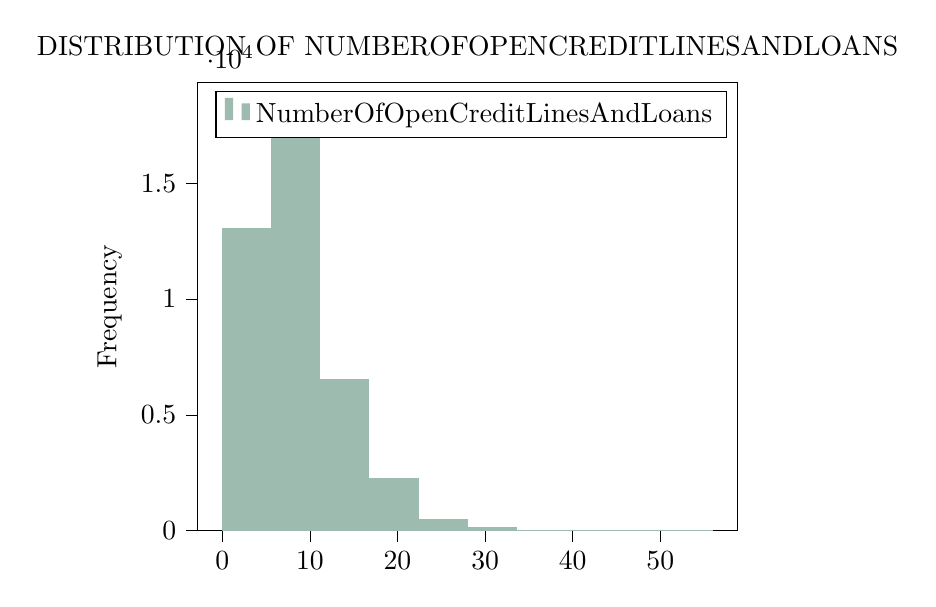
\begin{tikzpicture}

\definecolor{color0}{rgb}{0.615686274509804,0.733333333333333,0.682352941176471}

\begin{axis}[
tick align=outside,
tick pos=left,
title={\printsubsection{\MakeUppercase{Distribution of NumberOfOpenCreditLinesAndLoans}}},
x grid style={white!69.01960784313725!black},
xmin=-2.8, xmax=58.8,
xtick style={color=black},
y grid style={white!69.01960784313725!black},
ylabel={Frequency},
ymin=0, ymax=19370.4,
ytick style={color=black}
]
\draw[fill=color0,draw opacity=0] (axis cs:0,0) rectangle (axis cs:5.6,13063);
\addlegendimage{ybar,ybar legend,fill=color0,draw opacity=0};
\addlegendentry{NumberOfOpenCreditLinesAndLoans}

\draw[fill=color0,draw opacity=0] (axis cs:5.6,0) rectangle (axis cs:11.2,18448);
\draw[fill=color0,draw opacity=0] (axis cs:11.2,0) rectangle (axis cs:16.8,6541);
\draw[fill=color0,draw opacity=0] (axis cs:16.8,0) rectangle (axis cs:22.4,2283);
\draw[fill=color0,draw opacity=0] (axis cs:22.4,0) rectangle (axis cs:28,483);
\draw[fill=color0,draw opacity=0] (axis cs:28,0) rectangle (axis cs:33.6,141);
\draw[fill=color0,draw opacity=0] (axis cs:33.6,0) rectangle (axis cs:39.2,38);
\draw[fill=color0,draw opacity=0] (axis cs:39.2,0) rectangle (axis cs:44.8,8);
\draw[fill=color0,draw opacity=0] (axis cs:44.8,0) rectangle (axis cs:50.4,7);
\draw[fill=color0,draw opacity=0] (axis cs:50.4,0) rectangle (axis cs:56,4);
\end{axis}

\end{tikzpicture}